El diseño del dedo exoesqueleto con 6 GDL se muestra en la Figura \ref{fig:Diseno3D} en su 
posición inicial de "CASA" y está constituido por una cadena cinemática de 7 eslabones, que 
están todos conectados entre sí por articulaciones revolutas. El software que se utilizó para 
generar el diseño en 3D, fue solidworks porque tiene varias herramientas que ayudaron en el 
desarrollo matemático, así como su versatilidad para enlazarse con matlab, software con el que 
se programaron los cálculos.  

\begin{figure}[H]
    \centering
    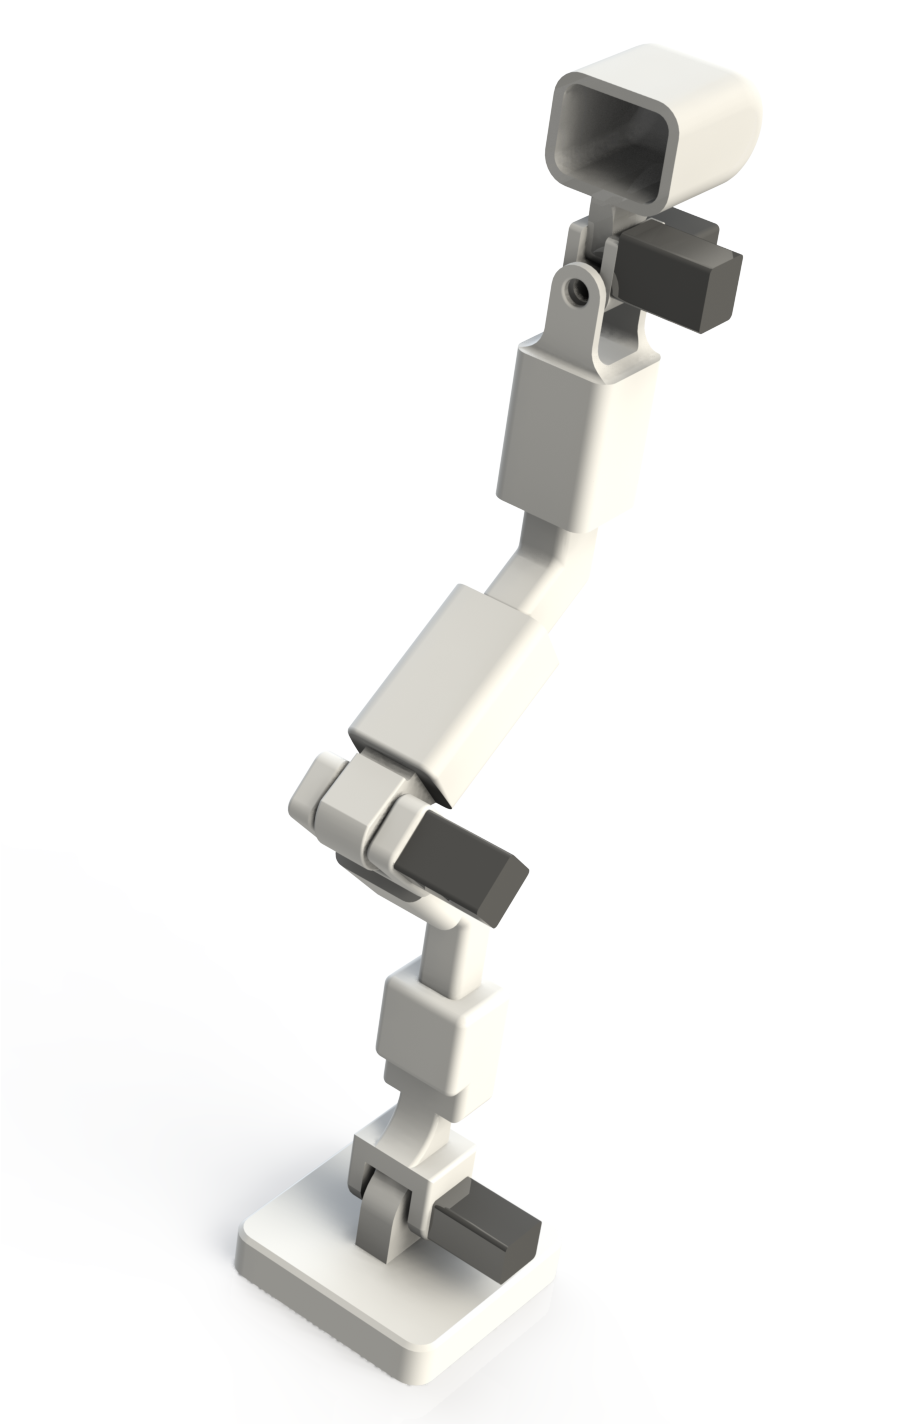
\includegraphics[scale=0.2]{Dedo Vist Isometrica.png} 
    \caption{Diseño 3D}
    \label{fig:Diseno3D}
\end{figure}

La disposición de las articulaciones que se muestran en la Figura \ref{fig:EsqArtOri}, fueron las 
planteadas en el trabajo HEXOTRAC: A highly Under-Actuated Hand Exoskeleton for Finger Tracking 
and Force Feedback (REFERENCIA).

\begin{figure} [H]
    \centering
    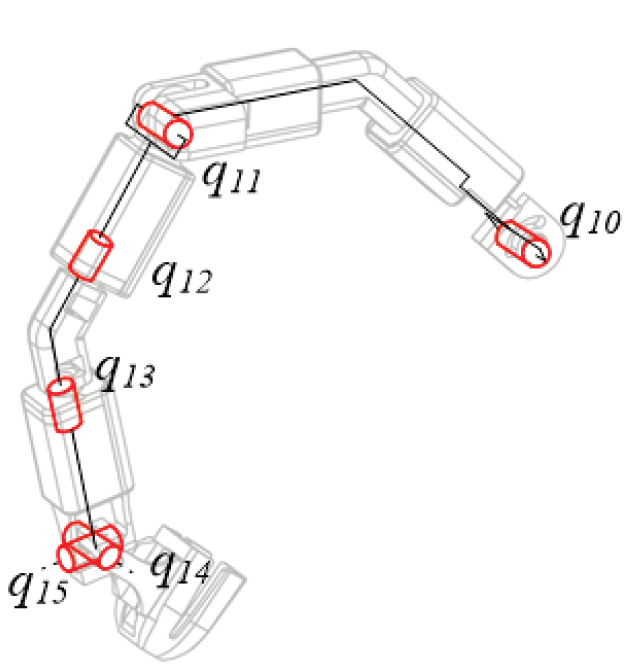
\includegraphics[scale=0.4]{EsquemaArticulaciones.png} 
    \caption{Esquema de las Articulaciones Original}
    \label{fig:EsqArtOri}
\end{figure}

Sin embargo por el equipo propuso una modificación y se agregó un eslabón más, de esta manera 
se evita que la articulación revoluta  $q_{14}$ y  $q_{15}$ estuvieran fusionadas, como se 
visualiza en la Figura \ref{fig:EsqArtOri}. El dibujo posicionado con una perspectiva lateral 
derecha, que se visualiza en la Figura \ref{fig:ExoPara} proporciona una imagen con dimensiones 
parametrizadas, mismas que se plasman en la siguiente tabla: 

\begin{table}[!ht] %[H]
    \centering
    \begin{center}
        \begin{tabular}{ccc}
        Parámetros & [m] \\
        \hline \hline 
        L1 & 0.03235525  \\ 
        L2 & 0.10513390  \\
        L3 & 0.02462267  \\
        L4 & 0.02228474  \\
        L5 & 0.04334075  \\
        L6 & 0.00600000  \\
        L7 & 0.01999013  \\
        L8 & 0.02565247  \\
        L9 & 0.01273194  \\
        L10 & 0.03641522 \\
        \end{tabular}
    \end{center}
\end{table}

Cabe destacar que el ángulo $\alpha$ que aparece en la imagen \ref{fig:ExoPara} es 
$\alpha$ = 59.26721315 [rad]. En la misma figura \ref{fig:ExoPara} se aprecia la asignación 
de referenciales $\Sigma_0$, $\Sigma_1$, $\Sigma_2$, $\Sigma_3$, $\Sigma_4$, $\Sigma_5$,  
$\Sigma_6$ y $\Sigma_7$. Los marcos inerciales propuestos a cada GdL se colocaron utilizando 
la convención GRyMA, manteniendo la dirección positiva de la mano derecha.

También se asignaron materiales, proponiendo para los eslabones un polímero termoplástico de 
nombre "acrilonitrilo butadieno estreno" también conocido como filamento ABS, utilizado por 
impresoras 3D, pensando que en un futuro próximo podamos imprimir el modelo y así experimentar 
con el en un entorno real. En el caso del dedal, se seleccionó un polímero artificial que 
pertenece al grupo de las poliamidas, llamado comunmente "Nylon", pues creemos que para cuidar 
la comodidad del usuario, al ingresar su dedo, el material no debe ser tan rígido y el nylon 
permite un equilibrio entre la suavidad y al mismo tiempo que no sea deformable.

Finalmente los motores propuestos son de micro Metal LP con reductora de 50:1, de corriente 
continua, con dimensiones de 24 x 10 x 12 mm y 10 gramos de peso. 

Al proponer materiales específicos, conocer sus dimensiones e incorporar las masas del motor 
pololu, se puede conocer el peso total del exoesqueleto, así como sus centros de masa 
(REFERENCIA TABLA 1 ANEXOS ) y los tensores de inercia de cada eslabón 
(REFERENCIA MATRICES EN ANEXOS), esta información se encuentra descrita en la sección de ANEXO  

\begin{figure}[H]
    \centering
    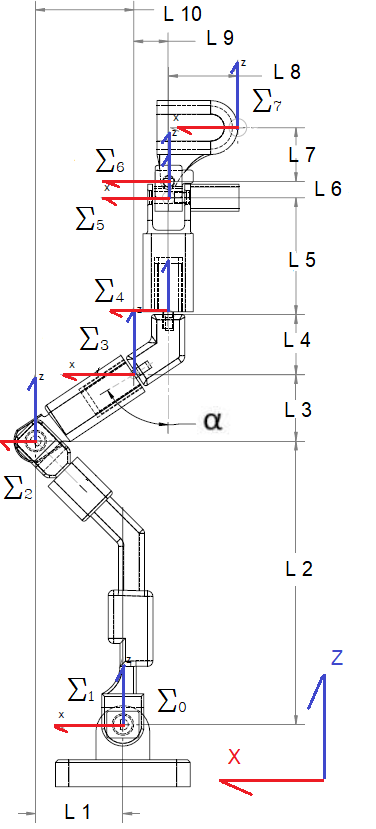
\includegraphics[scale=0.7]{ExoParametrizado.png}
    \caption{Esquema de las Articulaciones Utilizado}
    \label{fig:ExoPara}
\end{figure}

Conocer la cantidad de grados de libertar que tiene el exoesqueleto, nos servirá para identificar 
la versatilidad del movimiento que se podrá ejercer. Existen 3 clasificaciones [2]:

\begin{itemize}
    \item Menos de 6 GDL.  si el robot está diseñado para moverse en un espacio tridimensional, presentará  limitaciones su movimiento. 
    \item Exactamente 6 GDL. Se podrá mover de manera independiente en cada uno de los seis parámetros que conforman el espacio de trabajo tridimensional.
    \item Más de 6 GDL. Si un robot tiene más actuadores que los parámetros del espacio, implica que está sobre actuado.
\end{itemize}